\documentclass{article}
\usepackage{graphicx}
\usepackage[margin=1in]{geometry}
\usepackage[outdir=./]{epstopdf}  					% Avoids errors when input figures
\usepackage[labelsep=period,labelfont=bf]{caption}
%\usepackage{subcaption}

\begin{document}
	\begin{figure}[tbph]
		\caption{Response of 2-Year Advanced Country Yield to U.S. Monetary Policy Shocks} \label{fig:LPAE2Y}
		\begin{center}
			\begin{minipage}{\linewidth}
				\begin{center}
					\begin{subfigure}[t]{\linewidth}
						\includegraphics[trim={0cm 0cm 0cm 0cm},clip,height=0.24\textheight,width=\linewidth]{../Figures/LPs/LagDep-FX/Target/AE/TargetAEnomyptpphi24m.eps} \\
						\vspace{-0.35cm}
						\caption{Target Shock: 2000-2008} \label{subfig:LPAE2Ytarget}
						\vspace{0.4cm}
					\end{subfigure}
					
					\begin{subfigure}[t]{\linewidth}
						\includegraphics[trim={0cm 0cm 0cm 0cm},clip,height=0.24\textheight,width=\linewidth]{../Figures/LPs/LagDep-FX/Path/AE/PathAEnomyptpphi24m.eps} \\
						\vspace{-0.35cm}
						\caption{Path Shock: 2000-2019} \label{subfig:LPAE2Ypath}
					\end{subfigure}
					
					\begin{subfigure}[t]{\linewidth}
						\includegraphics[trim={0cm 0cm 0cm 0cm},clip,height=0.24\textheight,width=\linewidth]{../Figures/LPs/LagDep-FX/LSAP/AE/LSAPAEnomyptpphi24m.eps} \\
						\vspace{-0.35cm}
						\caption{LSAP Shock: 2009-2019} \label{subfig:LPAE2Ylsap}
					\end{subfigure}
				\end{center}
				\fignotes{This figure shows the response following \cite{Jorda:2005} of the 2-year advanced country nominal yield and its components to U.S. monetary policy shocks. The nominal yield is decomposed into an expected future short-term interest rate (ER) and a term premium (TP). The target, path and LSAP shocks are identified using high-frequency data around Fed's monetary policy announcements, see section \ref{sec:USMPS} for details.}
			\end{minipage}
		\end{center}
	\end{figure}
	
	\pagebreak[4]
	
	\begin{figure}[tbph]
		\caption{Response of 10-Year Advanced Country Yield to U.S. Monetary Policy Shocks} \label{fig:LPAE10Y}
		\begin{center}
			\begin{minipage}{\linewidth}
				\begin{center}
					\begin{subfigure}[t]{\linewidth}
						\includegraphics[trim={0cm 0cm 0cm 0cm},clip,height=0.24\textheight,width=\linewidth]{../Figures/LPs/LagDep-FX/Target/AE/TargetAEnomyptpphi120m.eps} \\
						\vspace{-0.35cm}
						\caption{Target Shock: 2000-2008} \label{subfig:LPAE10Ytarget}
						\vspace{0.4cm}
					\end{subfigure}
					
					\begin{subfigure}[t]{\linewidth}
						\includegraphics[trim={0cm 0cm 0cm 0cm},clip,height=0.24\textheight,width=\linewidth]{../Figures/LPs/LagDep-FX/Path/AE/PathAEnomyptpphi120m.eps} \\
						\vspace{-0.35cm}
						\caption{Path Shock: 2000-2019} \label{subfig:LPAE10Ypath}
					\end{subfigure}
					
					\begin{subfigure}[t]{\linewidth}
						\includegraphics[trim={0cm 0cm 0cm 0cm},clip,height=0.24\textheight,width=\linewidth]{../Figures/LPs/LagDep-FX/LSAP/AE/LSAPAEnomyptpphi120m.eps} \\
						\vspace{-0.35cm}
						\caption{LSAP Shock: 2009-2019} \label{subfig:LPAE10Ylsap}
					\end{subfigure}
				\end{center}
				\fignotes{This figure shows the response following \cite{Jorda:2005} of the 10-year advanced country nominal yield and its components to U.S. monetary policy shocks. The nominal yield is decomposed into an expected future short-term interest rate (ER) and a term premium (TP). The target, path and LSAP shocks are identified using high-frequency data around Fed's monetary policy announcements, see section \ref{sec:USMPS} for details.}
			\end{minipage}
		\end{center}
	\end{figure}
\end{document}
% trim = {<left> <lower> <right> <upper>}